\documentclass[a4paper,12pt]{article}
\usepackage[utf8]{inputenc}
\usepackage[top=2cm, bottom=2cm, left=3cm, right = 1.5cm]{geometry}
\usepackage[T2A]{fontenc}
\usepackage[english,russian]{babel}
\usepackage{amsmath,amsfonts,amstext,amssymb}
\usepackage{graphicx}
\bibliographystyle{plain}

\title{Учет неразрешенных двойных при оценивании массы рассеянных звездных скоплений}
%\author[1]{Don Joe}
%\author[1]{Static}
%\affil[1]{TeX.SX}
%
%\author{O. И. Бородина\inst{1}
%        \and
%        А. Ф. Селезнев\inst{1}
%        \and
%        Дж. Карраро\inst{2}
%        \and
%        А. М. Данилов\inst{1}
%          }
%          
%\institute{Уральский Федеральный Университет, ул. Мира 19, Екатеринбург\\

\author{О. И. Бородина$^1$ \and А. Ф. Селезнев$^1$ \and Дж. Карраро$^2$ \and В. М. Данилов$^1$ }

\date{\footnotesize{
    $^1$ Уральский Федеральный Университет, ул. Мира 19, Екатеринбург\\%
    $^2$ Dipartimento di Fisica e Astronomia, Universita’ di Padova Vicolo Osservatorio 3, Padova, Italy}\\% 
    }


\begin{document}
\maketitle
\section*{Реферат}
Одна из проблем, с которой сталкиваются исследователи звездных скоплений при оценивании их массы по функции светимости, это наличие в скоплении неразрешенных двойных систем. Особенно важно учитывать это обстоятельство при исследовании рассеянных звездных скоплений, где доля двойных может составлять десятки процентов. Цель настоящей работы - оценить, насколько учет неразрешенных двойных систем изменяет массу скопления.
 
В этой работе мы использовали функции светимости рассеянных звездных скоплений Ic2714, NGC 1912, NGC 2099, NGC 6834 и NGC 7142, которые были получены методом звездных подсчетов в ходе работы над созданием однородного каталога структурных и динамических характеристик рассеянных звездных скоплений по данным каталога точечных источников 2МАSS.

\section*{Введение}
Первые упоминания факта о наличии в звездных скоплениях большого количества неразрешенных двойных звезд можно обнаружить в работе Haffner \& Heckmann (1937) \cite{HH}.
С тех пор наличию двойных звезд было посвящено множество различных исследований. Например, Maeder в 1974 \cite{Maeder} показал, как располагается двойная на диаграмме звездная величина - показатель цвета в зависимости от отношения масс компонет $q=M_2/M_1$ (где $M_2$ это масса вторичной компоненты, а $M_1$ - масса главной компоненты двойной). В своей работе Hurley \& Tout (1998) \cite{HT} продемонстрировали, что последовательность, которая лежит выше главной последовательности звезд скопления на диаграмме CMD, образована двойными. Причем авторы этой работы выяснили, что коэффициент q имеет широкий разброс значений, то есть отношение масс компонент двойной может быть различным и может быть не равно 1 (что соответствует случаю одинаковых масс). 

Доля двойных звезд в шаровых звездных скоплениях относительно мала и обычно не превышает десяти процентов \cite{Milone2012} за несколькими исключениями. Однако, в работе Li с соавторами \cite{Li17} были обнаружены три шаровых скопления с гораздо большей долей двойных $(0.6-0.8)$

Рассеянные звездные скопления имеют значения доли двойных $\alpha \geqslant 30\%$ \cite{Li17, Boni, Khalaj, Sarro, alPer}. Этот процент все же меньше чем доля двойных среди звезд в окрестностях Солнца \cite{Duq1}. Было также получено, что доля двойных растет с увеличением массы главного компонента. Это чаще всего связано с динамической эволюцией звездного скопления \cite{KOP,Dorval}.

Очень важной характеристикой является функция распределения отношения масс компонент двойной $q$. В настоящее время среди исследователей нет точного согласия по поводу формы этого распределения. Согласно работе Duquennoy \& Mayor за 1991 год \cite{Duq2} функция распределения имеет максимум ближе к случаю маломассивных вторичных компонент, то есть далеко от 1. И наоборот, есть работы (например у Fisher с соавторами \cite{Fisher}), где пик расположен около случая равных масс компонент. Такой же пик был  обнаружен Maxted и другими \cite{Maxted} для маломассивных спектральных двойных в молодых скоплениях около $\sigma Ori$ и $\lambda Ori$. В работе Reggiani \& Meyer \cite{RM} была получена универсальная форма для распределения параметра $q$ для звезд типа Солнца и для карликов класса М в поле: $dN/dq \sim q^{\beta}$ с $\beta=0.25\pm0.29$. Это распределение можно считать плоским внутри интервала ошибок. 

Milone \cite{Milone2012} с соавторами определил, что  в интервале $q\in[0.5,1.0]$ распределение параметра $q$ у шаровых скоплений примерно плоское, с некоторыми отклонениями для нескольких случаев. А в работе Kouwenhoven и др. \cite{Kouwenhoven} использовались два других распределения: степенная зависимость $dN/dq \sim q^{\beta}$ для $q\in[q_0,1]$ и различных $\beta$, и Гауссово $dN/dq \sim exp[-(q-\mu_q)^2/2\sigma_q]$ для $q\in(0,1]$ с $\mu_q=0.23$ and $\sigma_q=0.42$.

Распределение отношения масс компонент двойной является ключом к восстановлению характеристик первоначальной популяции двойных. Было проведено множество численных исследований в данном направлении \cite{Kroupa2011,Geller2013,PR}.

Geller  и его соавторы \cite{Geller2013} показали на модели N-тел скопления NGC188, что распределение орбитальных параметров короткопериодичных двойных типа Солнца (с $P<1000^d$) должно быть примерно неизменным даже в пределах миллиарда лет эволюции. Это значит, что современные наблюдения двойных даже в старых скоплениях могут дать необходимую информацию о первоначальной их популяции. Parker \& Reggiani \cite{PR} показали, что общая доля двойных уменьшается в ходе динамической эволюции, но форма распределения $q$ не изменяется.  

Наличие неразрешенных двойных звезд в звездных скоплениях искажает оценки массы ЗС. Это следует учитывать как в случае звездных подсчетов, так и при оценке динамической массы (по значению дисперсии скоростей). Если набор звезд, отобранных по  оценке дисперсии скоростей (через лучевые скорости) содержит спектроскопические двойные, то значение дисперсии скоростей будет завышено. В результате, это приведет к завышенному значению массы скопления.

В работах Bianchini с соавторами \cite{Bianchini} и Kouwenhoven \& de Grijs \cite{KdeG} был сделан вывод, что учет населения двойных при оценке массы скопления очень важен. Селезнев с соавторами \cite{4337} отметили возможное влияние неразрешенных двойных на дисперсию скоростей, а затем и на оценку массы скопления NGC 4337

Когда масса скопления определяется через функцию светимости, полученную методом звездных подсчетов, то оценка массы будет меньше, чем в реальности, если не учитывать наличие в ЗС неразрешенных двойных. Это может быть легко объяснено тем, что масса двойной звезды больше массы одиночной с той же звездной величиной из-за сильной зависимости светимости звезд от их массы ($(L/L_{\odot})\sim(M/M_{\odot})^4$ \cite{CO}). 
Если одиночная звезда имеет ту же звездную величину, что и двойная, то их светимости также равны $L_s=L_1+L_2$ (где $L_s$ -- светимость одиночной звезды, а  $L_1$ и $L_2$ - светимости главного и вторичного компонента двойной соответственно). Тогда $M_s^4=M_1^4+M_2^4$, а значит $(M_1+M_2)^4=M_1^4+M_2^4+4M_1M_2^3+6M_1^2M_2^2+4M_1^3M_2=M_s^4+4M_1M_2^3+6M_1^2M_2^2+4M_1^3M_2$.
 Так как все величины положительные, то $(M_1+M_2)^4>M_s^4$, и $M_1+M_2>M_s$.
 
 Наличие неразрешенных двойных было учтено в работе Khalaj \& Baumgardt (2013) \cite{Khalaj} для оценки массы РЗС Ясли. Авторы определили долю двойных в скоплении -- $30\pm5$ процентов, а затем нашли поправочный коэффициент, равный 1.35 (чтобы учесть неразрешенные двойные в скоплении, следует умножить массу скопления, полученную в предположении, что все звезды в нем одиночные, на данный множитель). 
К сожалению, Khalaj \& Baumgardt \cite{Khalaj} не объяснили, каким образом был получено значение этого множителя. 

Сейчас мы планируем новый проект, который будет включать в себя оценки масс достаточно большого количества РЗС при помощи функции светимости. Тем самым, интересно выполнить оценку того, как корректирующий множитель зависит от доли двойных $\alpha$ и распределения $q$ в довольно большом интервале значений этих параметров. Это и является целью настоящей работы.

Она организована следующим образом: сначала  описывается принятая модель и используемый алгоритм, затем приводится описание и анализ результатов для пяти РЗС NGC 1912, NGC 2099, NGC 6834, NGC 7142, и IC 2714. 
	
	\section*{Модель и алгоритм}
Поправочный коэффициент к массе скопления зависит от двух параметров. Во-первых, необходимо учитывать распределение доли двойных по звездным величинам. В данном исследовании мы используем равномерное распределение, то есть доля двойных звезд одинакова для всех звездных величин, и имеет значения в интервале $10-90 \%$
Во-вторых, распределение параметра q может быть различным, в данной работы мы рассматриваем несколько видов распределений:
\begin{itemize}
	\item $\delta$ - функцию с $q = 1$
	\item плоское распределение
	\item Гауссово распределение из работы Kouwenhoven и др. \cite{Kouwenhoven}
	\item Гауссово распределение с модой, сдвинутой ближе к 1, чтобы воспроизвести результаты из работ Fischer и др. \cite{Fisher} и Maxted и др. \cite{Maxted}.
\end{itemize}

Математическое ожидание и стандартное отклонение последнего распределения имеют следующие значения: $\mu_q=0.60$ и $\sigma_q=0.42$.

Ранее уже рассматривали решения задач, связанных с моделированием двойных систем. Обзор таких работ был сделан Kouwenhoven \cite{Kouwenhoven} с соавторами и включает в себя следующие варианты постановки задач:

\begin{itemize}
	\item Случайное моделирование пары. Массы обоих компонентов случайным образом выбирается из распределения масс;
	\item Случайное моделирование пары, ограниченной главным компонентом. Масса главного компонента выбирается из распределения масс, затем выбирается масса звезды-спутника с требованием, чтобы она была меньше;
	\item Моделирование пары, ограниченный главным компонентом. Масса главного компонента выбирается из распределения масс, затем вычисляется масса звезды-спутника из распределения параметра $q$.;
	\item Расщепление ядра. Общая масса двойной системы берется из распределения масс. Масса главного компонента и звезды-спутника вычисляются по формулам связи массы системы и параметра $q$.
\end{itemize}
Наша задача отличается от решенных ранее, так как нам дана изначально звездная величина двойной системы, из которой мы должны определить массу компонентов. Таким образом, метод, описанный ниже, может быть назван <<моделированием пары, ограниченной общей светимостью>>.

Для того, чтобы связать массу и звездную величину, мы используем квадратичную функцию масса-светимость \ref{EkersEq} из работы Eker и др. \cite{Eker}:

\begin{equation}
\begin{array}{l}
\log{L} = - (0.705 \pm 0.041)(\log{M})^2  + (4.655 \pm 0.042) (\log {M}) - (0.025 \pm 0.010)\\
\label{EkersEq}
\end{array}
\end{equation}
где $L$ -- это светимость, выраженная в единицах светимости Солнца, а $M$  -- масса звезды, выраженная в массе Солнца.
 В своей работе Eker \cite{Eker} с соавторами получили еще и другие виды зависимостей, а также привели ряд аргументов, показывающих преимущество использования именно квадратичной формы.
 
 Выражение \ref{EkersEq} описывает одиночные звезды на главной последовательности, поэтому мы будем рассматриваем двойные, оба компонента которой находятся ниже точки поворота, и между которыми не происходит обмена веществом
 
Чтобы определить число звезд в интервалах звездных величин, мы используем функции светимости для рассматриваемых скоплений. Они были построены статистически на базе каталога 2MASS. Чтобы определить функцию светимости звезд скопления, мы сначала нашли функции светимости области скопления (<<скопление + фон>>) и диска той же площади вокруг этой области (<<фон>>). Предполагая, что фон одинаково однородный в обеих областях, мы вычли из функции светимости <<скопления + фон>> функцию светимости <<фона>> и получили функцию светимости скопления. Такая процедура была подробно описана в \cite{4337}.

Мы разбиваем функцию светимости скопления на одинаковые интервалы звездных величин $\Delta J$ (рисунок \ref{LF}), и в каждом из них считаем число звезд при помощи уравнения \eqref{Nstars} и число двойных \eqref{Nbstars} для заданной доли двойных $\alpha$.

\begin{equation}
N = \int\limits_J^{J+\Delta J}{F(J)dJ}
\label{Nstars}
\end{equation}

\begin{equation}
N_{b}=\alpha \int\limits_J^{J+\Delta J}{F(J)dJ}
\label{Nbstars}
\end{equation}

Мы округлили $N$ и $N_{b}$ до целых и вычислили $N_{s} = N - N_{b}$. В последствии для звезд одного промежутка $\Delta J$ мы будем использовать среднюю величину интервала.



\begin{figure}\centering
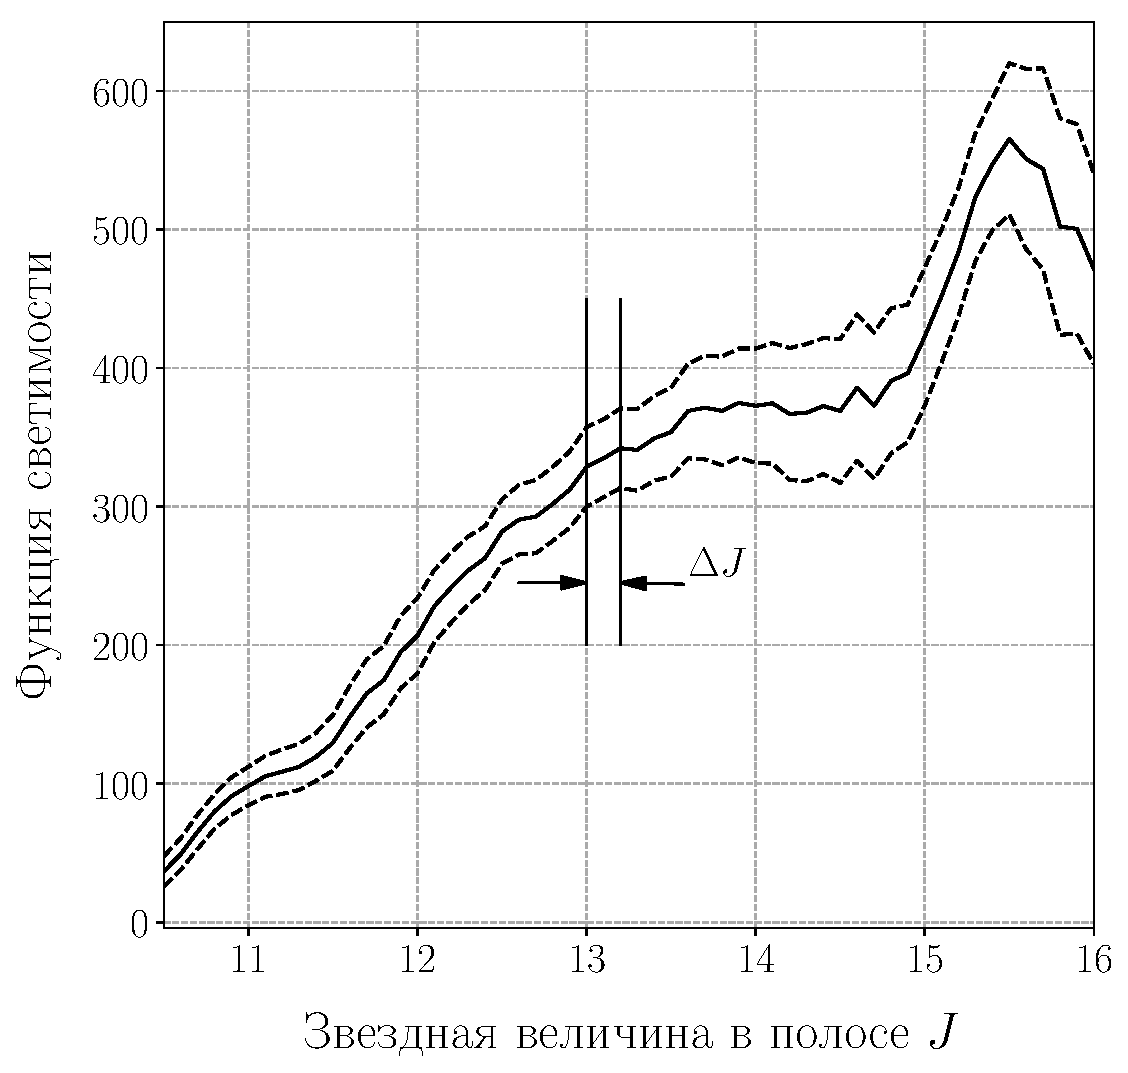
\includegraphics[width=7cm]{LF}
	\caption{Разбиение функции светимости (сплошная линия) скопления NGC 2099 на интервалы звездных величин. Пунктиром обозначен доверительный интервал функции светимости.}
	\label{LF}
\end{figure}

Затем мы переходим от звездной величины к массе, следующим образом. Сначала выбирается изохрона, которая соответствует возрасту скопления. Мы брали значение возраста из каталога Локтина и Поповой \cite{LoPo}, а затем уточняли, сравнивая с изохронами \cite{Bressan} диаграмму звездная величина-показатель цвета для отобранных звезд  скопления. Затем мы вычисляли абсолютные звездные величины, используя значения модуля расстояния и поглощения. Набор перечисленных параметров представлен в таблице \ref{clusters}. 

Зная абсолютную звездную величину звезд скопления, по таблице изохроны соответствующего возраста им можно сопоставить массы.  И теперь, с помощью формулы \ref{EkersEq} пересчитываем массу в значение светимости.

В таблицу \ref{clusters} также включили интервал масс, где минимальная масса соответствует звездной величине $J = 16^m$ (кроме скопления NGC6834, для которого из-за недостаточной полноты каталога 2МАSS взята $J = 15.9^m$ ), а максимальная масса определяется звездами, которые находятся у точки поворота (для ее определения мы использовали главную последовательность нулевого возраста).


\begin{table}[h!]
\caption{Параметры функций светимости скоплений}
\centering
		\begin{tabular}{|c|c|c|c|c|}
			\hline
				{Скопление} & {Интервал по $M, M_{\odot}$}& ${(m-M)_0}$ & \ ${E(B-V)}$ & ${\log(t)}$\\
			\hline
			IC2714 & [0.73; 2.82] & 10.48 & 0.34 & 8.6\\
			NGC1912 & [0.68;  3.60] & 10.29 & 0.25 & 8.3\\
			NGC2099 & [0.76;  2.77] & 10.74 & 0.30 & 8.7\\
			NGC6834 & [1.07;  5.12] & 11.59 & 0.71 & 7.9\\
			NGC7142 & [0.87;  1.80] & 10.2 & 0.25 & 9.2\\
			\hline
		\end{tabular}
\label{clusters}
\end{table}

 Затем мы построили 




	\newpage
	\bibliography{Biblyo}
\end{document}
